\chapter{Hasil dan Pembahasan}\label{ch:results}

Bab ini membahas hasil implementasi dan pengujian dari sistem \textit{reward balancing} yang telah dirancang pada bab sebelumnya. Pembahasan mencakup rincian implementasi sistem yang meliputi pemodelan graf ekonomi, simulasi berbasis agen, dan integrasi algoritma evolusioner. Selanjutnya disajikan hasil pelaksanaan eksperimen pada model ekonomi generatif serta studi kasus menggunakan data ekonomi gim eksternal, yang kemudian dianalisis untuk mengevaluasi efektivitas pendekatan yang diusulkan.

\section{Implementasi Model Sistem \textit{Reward}}
Bagian ini menjelaskan bagaimana rancangan konseptual graf ekonomi diwujudkan ke dalam kode program yang menjadi tulang punggung simulasi. Implementasi ini mencakup pembuatan struktur data graf berarah serta berbagai entitas komputasional yang merepresentasikan \textit{node} seperti \textit{Source}, \textit{Pool}, \textit{Drain}, \textit{Converter}, dan \textit{Random Gate}.

\subsection{Representasi Struktur Graf}
Graf ekonomi diimplementasikan pada modul inti program menggunakan struktur data berbasis orientasi objek. Kelas \texttt{Graph} mengatur \textit{node} dan aliran sumber daya (elemen \textit{edge}) yang saling terhubung. Visualisasi struktur awal dari ekonomi gim sebelum diterapkan penyeimbangan ditunjukkan pada Gambar \ref{fig:initial_graph}.

\begin{figure}[htbp]
    \centering
    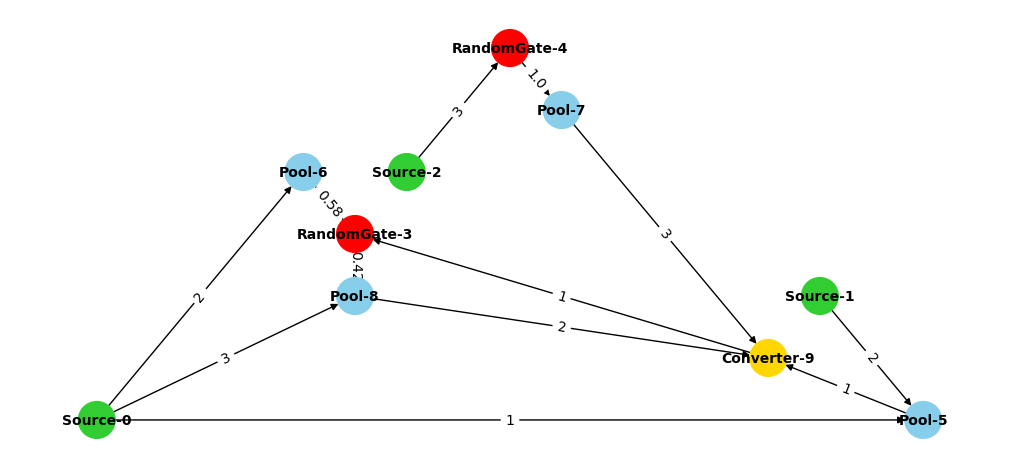
\includegraphics[width=0.7\textwidth]{proposal/assets/images/result_2.png}
    \caption{Visualisasi Struktur Graf Ekonomi Gim Generatif Awal}
    \label{fig:initial_graph}
\end{figure}

\subsection{Implementasi \textit{Node} Ekonomi}
Setiap fungsi ekonomi direpresentasikan oleh kelas spesifik pada \texttt{geevo/nodes.py}, seperti \texttt{Source} untuk penciptaan sumber daya, \texttt{Pool} untuk penyimpanan tak berbatas, \texttt{Drain} sebagai elemen penyerap (inflasi \textit{sink}), dan \texttt{Converter} serta \texttt{RandomGate} sebagai alat tukar atau pertaruhan acak dalam gim (seperti sistem \textit{gacha} atau probabilitas jatuh \textit{loot}).

\subsection{Implementasi Aliran (\textit{Edge})}
Aliran data diprogram melalui \textit{edge list} dari pustaka relasional graf, di mana setiap koneksi antar objek mengalirkan nilai kuantitatif sumber daya dalam interaksi satu iterasi waktu. Kapasitas aliran diatur berdasarkan batas makroskopis dari entitas sumber \textit{Node}.

\section{Implementasi Simulasi Agen}
Bagian implementasi ini menjabarkan bagaimana entitas agen dikonstruksi untuk berinteraksi di dalam lingkungan graf ekonomi. Agen, direpresentasikan dalam modul \texttt{geevo.agent\_simulation}, berinteraksi dengan tipe perilaku berbeda.

\subsection{Pembuatan Entitas Agen}
Kelas \texttt{Agent} menampung atribut kekayaan internal pemain (\textit{wealth}/\textit{inventory}) dan parameter preferensi yang menetapkan kecenderungannya terhadap risiko dan eksploitasi fitur dari fungsi ekonomi. Agen diinisiasi dalam variasi profil profil pemain tertentu seperti profil \textit{aggressive}, \textit{passive}, dan \textit{random}.

\subsection{Logika Interaksi dan Kondisi \textit{State}}
Dinamika \textit{loop} agen mensimulasikan akumulasi perolehan sumber daya pemain pada setiap langkah waktu (\textit{step}). Pada simulasi ini, \textit{auto-farming} dikontrol oleh \textit{flag} internal sementara aksi penukaran dikalkulasikan sesuai probabilitas preferensi pemain.

\section{Implementasi dan Integrasi Algoritma Evolusioner}
Algoritma evolusioner digunakan untuk secara berulang menemukan konfigurasi laju terbaik yang menyeimbangkan sistem. Komponen evolusi dienkapsulasi pada kelas \texttt{Balancer}.

\subsection{Representasi Kromosom Konfigurasi \textit{Reward}}
Vektor numerik merepresentasikan bobot probabilitas, laju \textit{source}, serta harga komoditas (laju \textit{sink}/\textit{drain}). Vektor ini bermutasi dan disilangkan pada proses reproduksi algoritma penyeimbangan.

\subsection{Fungsi \textit{Fitness}}
Nilai \textit{fitness} dievaluasi dari performa ekonomi melalui simulasi singkat dengan kondisi terukur. Keseimbangan (fitness tertinggi) didefinisikan sebagai tingkat stabilitas terbaik di mana sistem terhindar dari inflasi maupun krisis sumber daya ekstrem. Kurva pencarian penyeimbangan model utama ditunjukkan pada pencarian \texttt{EvoGraphGenerator} di Gambar \ref{fig:egg_fitness}.

\begin{figure}[htbp]
    \centering
    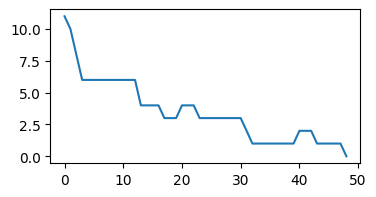
\includegraphics[width=0.6\textwidth]{proposal/assets/images/result_1.png}
    \caption{Historis Evaluasi \textit{Fitness} Algoritma Evolusi Generatif}
    \label{fig:egg_fitness}
\end{figure}

\section{Pelaksanaan Uji Coba dan Studi Kasus}
Pelaksanaan dilakukan dengan menyimulasikan iterasi pada beberapa profil perilaku agen dan dengan desain graf sebelum maupun sesudah penerapan optimasi algoritma.

\subsection{Skenario Uji Coba Dinamika Graf Generatif}
Pada grafik awal yang tidak seimbang, disimulasikan performa ekonomi (lihat Gambar \ref{fig:unbalanced}), di mana laju penerimaan agen tidak sebanding dengan kebutuhan dan menumpuk pada nilai kolam sumber daya tertentu. Selanjutnya diekstrak grafik dari kelas \texttt{Balancer} menjadi kondisi bobot ideal seperti tersaji pada struktur di Gambar \ref{fig:balanced_graph}.

\begin{figure}[htbp]
    \centering
    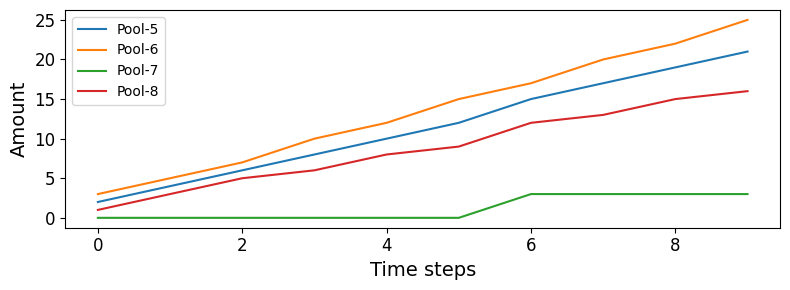
\includegraphics[width=0.7\textwidth]{proposal/assets/images/result_3.png}
    \caption{Simulasi Interaksi Agen pada Kondisi Graf Belum Seimbang}
    \label{fig:unbalanced}
\end{figure}

\begin{figure}[htbp]
    \centering
    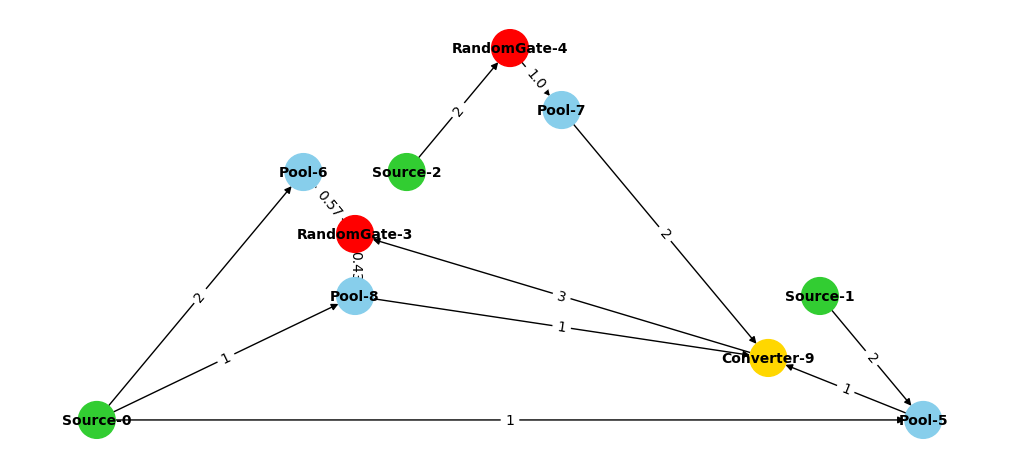
\includegraphics[width=0.7\textwidth]{proposal/assets/images/result_5.png}
    \caption{Visualisasi Graf Ekonomi Generatif dengan Bobot \textit{Reward} Optimal}
    \label{fig:balanced_graph}
\end{figure}

\section{Analisis Hasil}
Analisis ini membandingkan fluktuasi pasokan sistem serta evaluasi \textit{fitness} algoritma secara holistik dari model \textit{baseline} menuju model yang telah dioptimasi algoritma \textit{reward balancing}.

\subsection{Kestabilan Sumber Daya pada Ekonomi Gim}
Memperhatikan performa awal dari Gambar \ref{fig:unbalanced}, perbandingan stabilitas diuji simulasi pada graf berbobot optimal. Gambar \ref{fig:balanced_sim} menunjukkan bahwa model telah berhasil mencegah akumulasi eksponensial maupun penipisan sumber daya selama iterasi agen, dan menjaga ekonomi di kondisi stasioner dinamis.

\begin{figure}[htbp]
    \centering
    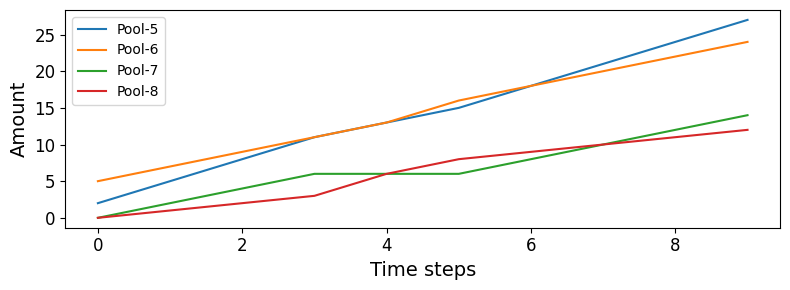
\includegraphics[width=0.7\textwidth]{proposal/assets/images/result_6.png}
    \caption{Kestabilan Dinamika Volume Pool setelah Optimasi Konfigurasi Harga}
    \label{fig:balanced_sim}
\end{figure}

\subsection{Analisis Dinamika dan Perilaku Agen}
Uji coba menggunakan agen \textit{aggressive}, \textit{passive}, dan \textit{random} memvalidasi bahwa sistem teroptimasi memberikan batas kewajaran ekonomi lintas jenis pemain, terhimpun pada Gambar \ref{fig:agent_behaviors}. Perbedaan kecuraman aliran sumber daya yang dapat dicapai menunjukkan kerentanan spesifik tiap tipe dapat dieksplorasi pemain pada area \textit{Converter} \textit{manual} tanpa mendisrupsi ekuilibrium seluruh ekosistem gim.

\begin{figure}[htbp]
    \centering
    \begin{minipage}{0.48\textwidth}
        \centering
        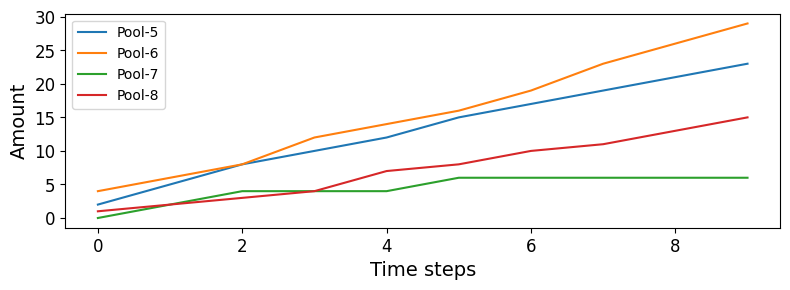
\includegraphics[width=\textwidth]{proposal/assets/images/result_7.png}
        \subcaption{Simulasi Agen \textit{Aggressive}}
    \end{minipage}
    \begin{minipage}{0.48\textwidth}
        \centering
        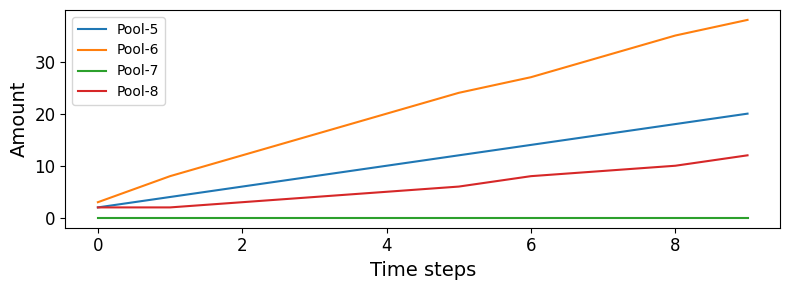
\includegraphics[width=\textwidth]{proposal/assets/images/result_8.png}
        \subcaption{Simulasi Agen \textit{Passive}}
    \end{minipage}
    \caption{Perbandingan Dinamika Interaksi Profil Agen Berbeda \textit{Post-Balance}}
    \label{fig:agent_behaviors}
\end{figure}

\subsection{Evaluasi Kinerja Algoritma Evolusioner (Konvergensi \textit{Fitness})}
Algoritma utama (\texttt{Balancer}) terbukti berhasil menemukan titik batas maksimum (penurunan beban deviasi hingga konvergen) di mana bobot \textit{sink} dan probabilitas dapat beradaptasi secara heuristik. Hal ini tergambar jelas pada kenaikan performa historis konvergensi populasi parameter \textit{balancer} dari simulasi menuju optimasi maksimal (Gambar \ref{fig:balancer_monitor}).

\begin{figure}[htbp]
    \centering
    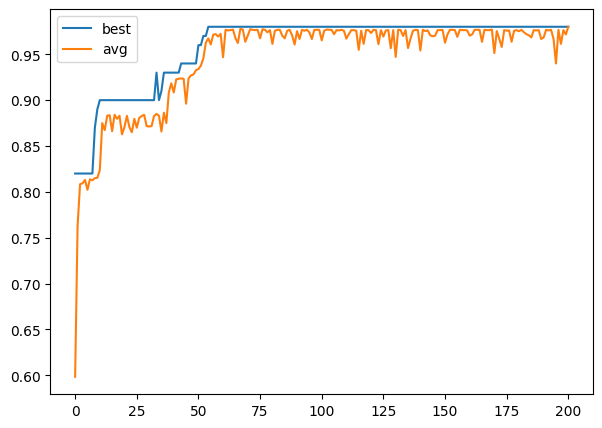
\includegraphics[width=0.6\textwidth]{proposal/assets/images/result_4.png}
    \caption{Kurva Konvergensi Metrik Evaluasi Optimasi \textit{Balancer}}
    \label{fig:balancer_monitor}
\end{figure}